\documentclass[review]{elsarticle}

\usepackage{lineno,hyperref}
\modulolinenumbers[5]

\usepackage[top=2.54cm, bottom=2.54cm, left=2.54cm, right=2.54cm]{geometry}
\usepackage{amsmath}
\usepackage{graphicx}
\usepackage{subfig}
\renewcommand{\thesubfigure}{\Alph{subfigure}}% uppercase subfloat numbering
\graphicspath{{../figures/}}


\journal{Journal of Theoretical Biology}

%%%%%%%%%%%%%%%%%%%%%%%
%% Elsevier bibliography styles
%%%%%%%%%%%%%%%%%%%%%%%
%% To change the style, put a % in front of the second line of the current style and
%% remove the % from the second line of the style you would like to use.
%%%%%%%%%%%%%%%%%%%%%%%

%% Numbered
%\bibliographystyle{model1-num-names}

%% Numbered without titles
%\bibliographystyle{model1a-num-names}

%% Harvard
%\bibliographystyle{model2-names.bst}\biboptions{authoryear}

%% `Elsevier LaTeX' style
\bibliographystyle{elsarticle-num}
%%%%%%%%%%%%%%%%%%%%%%%

\begin{document}

\begin{frontmatter}

\title{Neural crest migration with continuous cell states}

%% Group authors per affiliation:
\author{Linus J. Schumacher\fnref{myfootnote}}
\address{MCR Centre for Regenerative Medicine, University of Edinburgh}
\ead{Linus.Schumacher@ed.ac.uk}


\begin{abstract}
Models of cranial neural crest cell migration in cell-induced (or self-generated) gradients have included a division of labour into leader and follower migratory states, which undergo chemotaxis and contact guidance, respectively. Despite validated utility of these models through experimental perturbation of migration in the chick embryo and gene expression analysis showing relevant heterogeneity at the single cell level, an often raised question has been whether the discrete cell states are necessary, or if a continuum of cell behaviours offers a functionally equivalent description. Here we argue that this picture is supported by recent single-cell transcriptome data. Motivated by this, we implement two versions of a continuous state model: (1) signal choice and (2) signal combination. We find that migration is more persistent than in the discrete state model and than in experimental observations. We further show that the signal combination model, but not the signal choice model, can be successfully adjusted to experimentally plausible regimes by reducing the chemoattractant consumption parameter. Thus we show an equivalently plausible, experimentally motivated, model of neural crest cell migration.
\end{abstract}

\begin{keyword}
collective behaviour \sep cell migration \sep developmental biology
\MSC[2010] 92C15
\end{keyword}

\end{frontmatter}

\linenumbers

\section{Introduction}
Neural crest cell migration is a popular example of collective cell behaviour in development. Neural crest cells migrate over long distances in the vertebrate embryo and contribute to a variety of tissue types. Understanding their migration is important to identify the causes for birth defects, and they also provide a model system to study the invasive migration of cancer cells, especially the neural crest derived melanoma \cite{Kulesa2006,Bailey2012,McLennan2017}. Mechanisms of neural crest cell migration have been studied in a variety of model organisms, and multiple groups have approached the problem with mathematical modelling \cite{Simpson2007,Landman2011,Carmona-Fontaine2011,Wynn2012,Wynn2013,McLennan2012,McLennan2015,Mort2016,Zhang2018,Merchant2018}. %% longer?

Previous work has shown that chick cranial neural crest cell migration can be described with discrete leader-follower states that alternatively undergo chemotaxis or contact-guidance \cite{McLennan2012,McLennan2015}, and switch between the two on a non-zero timescale based on VEGF signals \cite{McLennan2015b}. The utility of this model has been validated in a number of ways, such as using the model to predict the outcome of tissue transplantation experiments \cite{McLennan2012,McLennan2015,McLennan2015b}, and gene expression analysis \cite{McLennan2015,McLennan2015b}, including recent single-cell RNAseq \cite{Morrison2017}. While earlier studies identified key differences between neural crest sub-groups for selected genes, the advent of single-cell whole transcriptome analysis provides an opportunity to investigate the heterogeneity of the neural crest subpopulation in a less biased way. %% more specific?

What has hitherto not been investigated is whether leader-follower cell states need be discrete, or could lie on a continuum. This question is relevant in light of ongoing debate in the literature about whether mechanisms of neural crest cell migration are common or distinct in different model organisms \cite{Schumacher2016a,Richardson2016,Genuth2018}. Here theoretical biology can provide a useful argument, due to the difficulty of inferring heterogeneity from cell tracking data alone \cite{Schumacher2017}. From a molecular perspective, such questions about cellular identity are now just coming within reach of experimental measurement \cite{Wagner2016}, making this a highly timely topic of enquiry. %% more specific?

Here we address whether chick cranial neural crest cell migration can be described with continuous cell states equally well as existing models and with experimentally plausible outcomes. We first revisit recently published single-cell transcriptome data \cite{Morrison2017} to show that a continuum of cell states is not ruled out by the data. We then modify previous models \cite{McLennan2015,McLennan2015b} to assess what effect a continuum of cell guidance behaviours has on the collective migration, providing two alternative implementations of choosing between chemotaxis and contact guidance, or combining information from both signals. We find that the naive implementation of continuous states achieves unrealistic migration outcomes with cells migrating too far, and explore how the models can be modified to remedy this without sacrificing total cell number. The signal combination model can be successfully adjusted by reducing the chemoattractant consumption rate, thus providing a reasonable alternative (or equivalent) to the model of discrete leader and follower states. We finish by discussing model robustness and plausible alternative modifications. % rephrase?

\section{Results}
\subsection{Analysis of single-cell gene expression}
Previous models have shown that migration in a cell-induced gradient can be more successful with fewer cells in a leader state, suggesting heterogeneity of cell states at the scale of a few or tens of cells, which has been confirmed with RT-qPCR \cite{McLennan2015}. Recently published single-cell RNAseq data \cite{Morrison2017} is a less biased way to measure the heterogeneity of gene expression in a cell population, as it measures the whole transcriptome instead of selected genes. The published analysis of this dataset focussed on the identification of gene-signatures based on the pairwise differential expression between groups, such as cells from trailing, lead, and front portions of the migratory stream \cite{Morrison2017}. An alternative approach is to explore the data with the question of whether cell states may be discrete or continuous.

Analysis of single-cell transcriptomes is challenging because many (thousands) genes are sampled and cell numbers can be low (hundreds), particularly when they have to be individually dissected. Here we utilize an approach from random matrix theory that discerns how many principal components of a data-set can be expected to result from non-random correlations given the size of the data set. This approach has previously been used for single-cell gene expression analysis\cite{Klein2015a}, and recently published as a software tool \cite{Aparicio2018} to separate out the signal from the noise in the variation of gene expression between cells. In the neural crest data set \cite{Morrison2017}, we focus on in vivo cells from chick embryo stages HH13\&15, were we have cells from trailing, lead, and invasive front portions of the stream. We find that 59 dimensions are non-trivial (Fig.~\ref{figMP}). The resulting 59-dimensional dataset is mapped to two dimensions using a force-based embedding approach \cite{Weinreb2018}. Labelling cells according to where in the stream they were sampled from, this exploratory visualisation of the population structure broadly maintains the order of spatial positions in the stream of trail, lead, front (Fig.~\ref{figscRNAseq}). There is further structure visible in the data, with the possible existence of subgroups comprising all three sample categories, which we don't investigate further here. Overall, there is mixing and overlap between the sample categories, but with a discernible ordering, which supports the view that cell states may be continuous.

\begin{figure}
    \centering
    {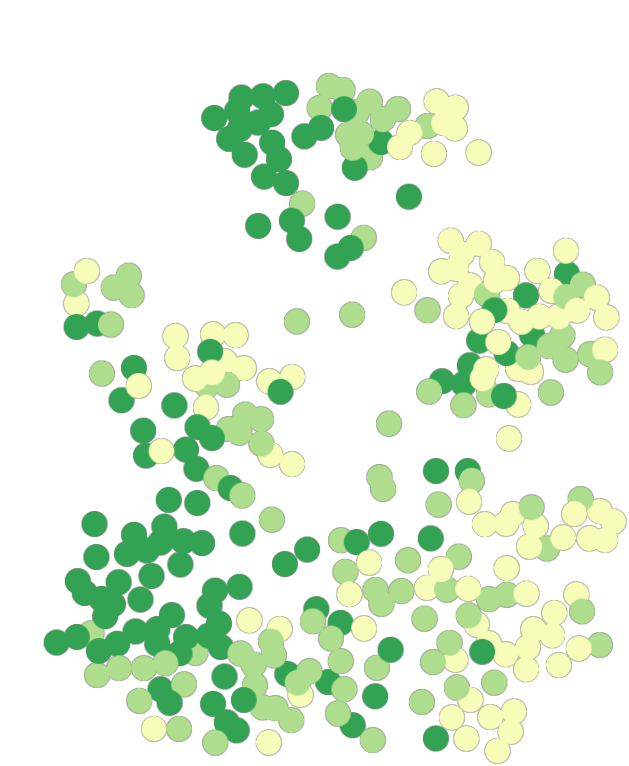
\includegraphics[scale=0.25]{Neural_Crest_NC_59PCs_HH1315}}
    \caption{Visualisation of a continuum of neural crest cell states. Single-cell RNAseq data \cite{Morrison2017} from chick cranial neural crest (Hamburger-Hamilton stages 13 and 15, 310 cells in total) taken from distinct locations in the migratory stream (trail: dark green, lead: light green, invasive front: pale yellow) were projected onto two dimensions for visualisation using a force-based embedding method \cite{Weinreb2018}. Only the top 59 principal components (out of 14299 genes measured, 12909 after preprocessing) were retained prior to embedding, based on random-matrix analysis \cite{Aparicio2018} (Fig.~\ref{figMP}).\label{figscRNAseq}}
\end{figure}

\subsection{Model of neural crest cell migration}% add a brief model description
Motivated by our exploratory analysis of single-cell RNAseq data, we wanted to investigate what effect a continuum of leader and follower migratory behaviours would have on the collective migration of neural crest cells. We built upon the existing model developed by the author and others \cite{McLennan2012,McLennan2015,McLennan2015b}, which we briefly describe here: The model is a 2D hybrid model with agent-based cell movement and a reaction-diffusion equation for the chemoattractant, solved on a growing domain, with the cells acting as sink-terms, resulting in a cell-induced, or self-generated gradient in the otherwise uniform chemoattractant. Cells enter the domain on one side, obeying volume exclusion, and sample discrete number of directions (representing filopodia) to look for favourable chemoattractant gradients or contact guidance, depending on whether they are in a leader of follower state. Cells can switch between these discrete states on a non-zero timescale \cite{McLennan2015b}, which is controlled by the continued exposure the chemoattractant gradient signal. Further modifications of this model introduced an inhibitory zone that can slow down cells and hence improve stream cohesion \cite{McLennan2017}, but we have not used this here. Previous versions of the model have implemented no-flux boundary conditions for the cells at the edge of the migratory domain. Here we instead adopt reflective boundary conditions that prompt cells to move away from the boundary, to more accurately represent the inhibitory zones  \cite{Kulesa2010,Szabo2016a} that are thought to shape or confine the stream of cells. The change in boundary condition mainly changes the stream morphology (cells don't stay very close to the boundary), but do not effect the overall migration profiles.

\subsubsection{Signal choice model}
One alternative to discrete cell states that are restricted to make use of either chemotaxis or contact guidance (Fig.~\ref{figNaiveModel}A), is that each cell can choose between these two signals (Fig.~\ref{figNaiveModel}B). This model reflects the hypothesis that cells can sense both signals, but only act on one or the other at a given time. This is implemented by a stochastic choice between the two signals, where the probability is given by the strength of the gradient signal. For simplicity, we have here chosen a linear relationship $P_{ch} = \Delta c$, where $\Delta c$ is the magnitude of the chemoattractant gradient measured between the cell body and its filopodial tip. This quantity is bounded between 0 and 1 and the chemoattractant concentration in our model is set in arbitrary units between 0 and 1. The contact guidance signal is thus chosen with a probability of $P_{cg} = 1 - \Delta c$. Thus a cell's direction of movement, $\vec{\theta}$, is given by
\begin{equation}
     \vec{\theta} = 
         \begin{cases}
         \vec{\theta}_{ch}, & P_{ch} = \Delta c \\
        \vec{\theta}_{cg}, & 1 - P_{ch}
        \end{cases}
\end{equation}
where $\vec{\theta}_{ch}$ is the direction of the (sampled) chemoattractant gradient signal, and $\vec{\theta}_{cg}$ is the direction prescribed by contact guidance.

\subsubsection{Signal combination model}
A second possibility for continuous states is that each cell combined the directional information from chemotaxis and contact guidance (Fig.~\ref{figNaiveModel}C). This reflects the hypothesis that both signals generate a motile force in the cell's cytoskeletal machinery, and the cell moves in the resulting overall direction. We implement this by setting a cells direction of movement as a weighted sum of the directions from contact guidance and chemotaxis, with the weighting determined by the strength of the gradient signal. For simplicity we have again chosen a linear weight, such that the overall direction is given by 
\begin{equation}
	\vec{\theta} = \Delta c\ \vec{\theta}_{ch} + (1 - \Delta c)\vec{\theta}_{cg},
\end{equation}
with the individual directions as above.

\begin{figure}
    \centering
    \subfloat[]{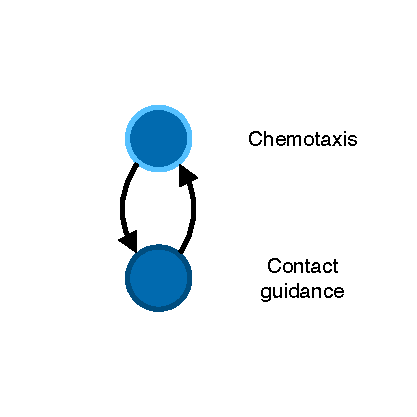
\includegraphics[]{modelSchematicControl}}
    \subfloat[]{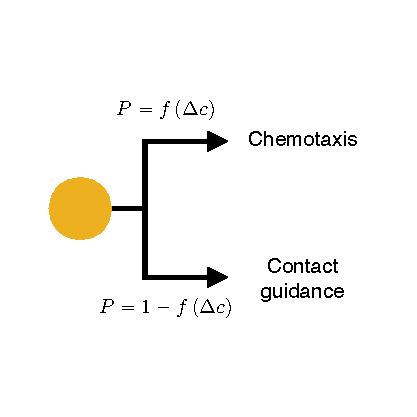
\includegraphics[]{modelSchematicChoice}}
    \subfloat[]{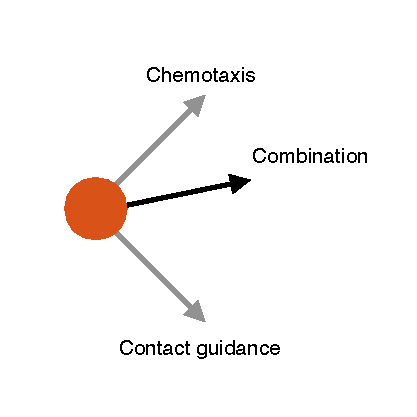
\includegraphics[]{modelSchematicCombination}}\\
    \subfloat[]{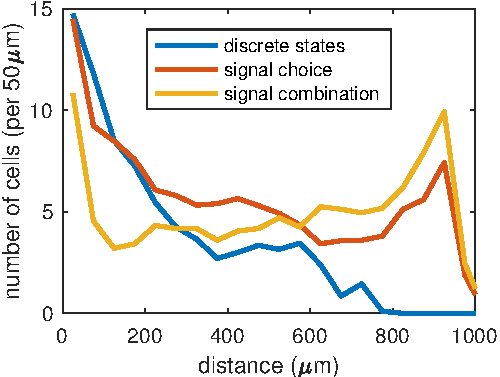
\includegraphics[]{Fig2_contStates_combination_sensAcc_10}}
    \subfloat[]{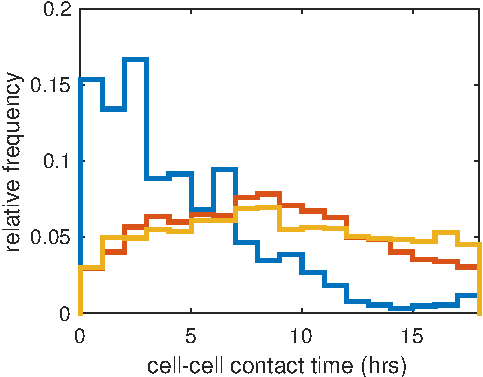
\includegraphics[]{Fig2B_contStates_combination_sensAcc_10}}
    \caption{Comparison of collective cell migration models with discrete and continuous states. (A) In the previously published model \cite{McLennan2015b}, cells switch between migratory states based on the presence of a chemotactic signal and at a non-zero timescale. (B) In the signal choice model, cells choose between chemotaxis and contact guidance for their direction of movement, with a probability related to the strength of the gradient signal. In results shown here, we have used $P_\mathrm{ch}=\Delta c$ for chemotaxis and $P_\mathrm{cg}=1 - \Delta c$ for contact guidance. (C) In the signal combination model, cells combine the directional information from both chemotaxis and contact guidance, with a weighting depending on the strength of the gradient signal. Here we have used a linear weight of $\Delta c$. (D) Migration profiles of the three models after 18h of migration. (E) Durations of cell-cell contacts during migration for the three models. Line colours as in (D). (C,D) Data shown are averages over 20 simulations for the discrete state model, and 40 simulations for each of the signal choice and signal combination models. \label{figNaiveModel}}
\end{figure}

\subsection{Continuous states migrate further than discrete states}
To compare the original model with its two alternatives, we simulate migration for 18h and visualise the result as a histogram of number of cells vs distance migrated. Both the signal choice and signal combination models migrate further than the discrete state model (Fig.~\ref{figFurtherModel}D), and further than is typically observed experimentally. This can be interpreted as the cells have more directional information to act on and hence being able to migrate in a more directed manner towards the target zone at the end of the migratory route. We further observed that in this implementation of the continuous state model, cells stay attached to each other longer (Fig.~\ref{figFurtherModel}E), whereas previously leaders would not engage in contact guidance at all, and thus cells would detach when switching from the follower to the leader state. In the continuous state model, cells can instead stay attached to their nearby neighbours throughout migration, even if primarily undergoing chemotaxis. We thus considered two avenues to refine this initial implementation, by either breaking long-term cell-cell contact or affecting the gradient sensing. % mention/show stream break-up?
% reference for filopidal-cell contact times? (on the order of hrs)

\subsection{Reducing contact guidance persistence reduces cell number and distance migrated}
To prevent the unrealistically long filopodia-cell contact times observed in the continuous state models (Fig.~\ref{figFurtherModel}E), we allowed a cell's filopodia to detach stochastically from the cell it is in contact with, with probability $P_d$ at every time-step. We then varied the detachment probability to assess whether a reduction in the distance migrated could be achieved without a large loss in the total cell number, as this represents the experimentally plausible scenario in unperturbed in vivo migration. Simulation results show that increasing the detachment probability in either the signal choice or signal combination models (Fig.~\ref{figFurtherModel}A) does decrease the distance migrated, but also rapidly decreases total cell number. Hence, reducing the persistence of contact guidance is insufficient to make the continuous state models biologically plausible.

\begin{figure}
\centering
\subfloat[]{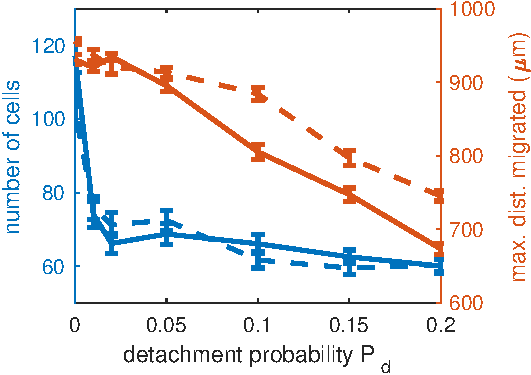
\includegraphics[]{Fig3_contStates_Psa_sensAcc_10}}\
\subfloat[]{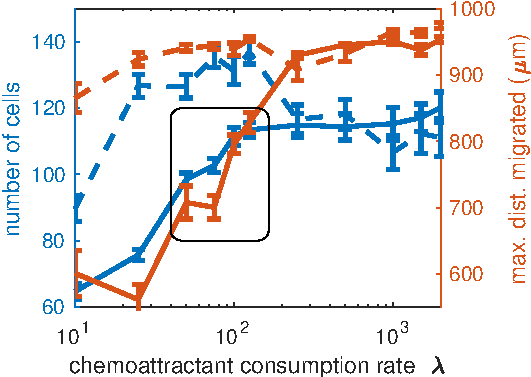
\includegraphics[]{Fig3_contStates_eat_sensAcc_10}}
\caption{Modifications to the continuous-state models can achieve experimentally realistic results. (A) Introducing a detachment probability, $P_d$, for the filopodial contacts used for contact guidance decreases the maximum distance migrated, but only at the cost of decrease total cell number for both the signal choice model (dashed lines) and the signal combination model (solid lines). (B) Reducing the chemoattractant consumption rate, $\lambda$, to the range of 40-150 (arbitrary units per hour) achieves realistic maximum distances migrated, with only a moderate reduction in cell number (highlighted by the black rectangle) for the signal combination model (solid lines), but not the signal choice model (dashed lines). Data shown are averages over 40 simulations for each parameter value, error bars show standard error of the mean.\label{figFurtherModel}}
\end{figure}

\subsection{Shallower cell-induced gradients enable the signal combination model}
We reasoned that affecting the model parameters relating to the chemoattractant may make the cell migration in the continuous state models less directed. Reducing the chemoattractant consumption, $\lambda$, of the cells decreases the sink-term in the reaction-diffusion equation, and should hence create shallower local gradients in the chemoattractant. When we reduced this parameter in our simulations, the distance migrated decreases before the total cell number for the signal combination model, and achieved experimentally observable values for the range 40-150 (arbitrary units per hour) (Fig.~\ref{figFurtherModel}B). This was not the case for the signal choice model. The behaviour is otherwise robust for wide ranges of the experimentally less-constrained parameter values, chemoattractant diffusivity and background production (Fig.~\ref{figNaiveModelSweeps}A\&B), with the exception of very high chemoattractant diffusivity in the combination model, which showed low cell numbers. 
% cite Insall?

\section{Conclusions}
We have revisited the model of chick cranial neural crest migration to address the question whether leader/follower (chemotaxis/contact guidance) cell migratory states could be continuous rather than discrete (Fig.~\ref{figNaiveModel}A). This was motivated in part by debates in the field, and in part by the recent availability of transcriptome data at single cell resolution. We reanalysed published gene expression data and found that this can support a continuum of cell states (Fig.~\ref{figscRNAseq}). Starting from our previous cell migration model, we then implemented two versions of a continuous state model, in which cells either choose between directional signals (Fig.~\ref{figNaiveModel}B) or combine the directional information (Fig.~\ref{figNaiveModel}C). The initial implementations of these models, without any further modifications, showed more persistent migration than the discrete state model (Fig.~\ref{figNaiveModel}D), with the distance migrated overshooting experimentally observed values. By changing the chemoattractant consumption, a key parameter that determines the cell-induced/self-generated gradient, we able to rescue the signal combination model to achieve experimentally observed migration distances without an unreasonably reduction in total cell number.

%\paragraph{need other methods for dealing with various sources of noice in single cell data to decompose ``vectors of cellular identity'' \cite{Wagner2016}}

It is possible that other model modifications would have had a similar effect. We could have chosen a non-linear relationship for the weighting in combining chemotaxis and contact guidance. Further to this, one could refine the model by making the chemoattractant consumption proportional to a cells ``leaderness'', based on the experimental observation that VEGF receptor expression is higher in cells at the invasive front \cite{McLennan2015,Morrison2017}. Based on our assessment presented here, the stochastic choice model is less plausible than the combination model. The role of stochasticity has also been investigated in other aspects of neural crest migration, such as colonisation of the gut \cite{Binder2015,Smadbeck2015,Zhang2018} and pigmentation patterning \cite{Mort2016}, and one could further explore the role of noise in contact guidance, for example by adding angular noise to the directional signal sensed, which we would expect to reduce the persistence of migration. Extending the model to 3D could also reduce distance moved in the primary direction of migration, as more of the movement would be along the other two dimensions. We can readily conceive of other versions of a continuous state model that may be realistic presentations of the neural crest migration, our work shows at least one such example, and that continuous state models ought to be taken into account.

The comparison with experimental data in these models has been largely semi-quantitative due to the limitations in quantifying relevant statistics such as total cell number and distance migrated. Distance migrated is not absolutely quantified experimentally, due to embryo-to-embryo size variation, and a missing consensus on what to measure as a start-point. Further difficulties arise due to the incomplete labelling efficiency of electroporated fluorescent markers. The time over which cell-cell contacts mediating contact guidance persist has not been quantified across the whole migratory population, yet long-contacts in the continuous state models seem unrealistic. Thus the model points to avenues for further experimental quantification, which in turn would constrain our models. % rephrase? reference electroporation efficiency? reference contact-time?

Alternatives to the chemotaxis and contact guidance paradigm have been put forward in related work. Contact-inhibition of locomotion has been studied as a mechanism enabling collective migration both in computational models and in \textsl{Xenopus} embryos \cite{Carmona-Fontaine2011}, but this has not been observed in chick cranial neural crest \cite{Genuth2018}. Another alternative to contact guidance would be pulling of followers by leader cells \cite{Yates2018}, and vice versa, which would improve overall stream cohesion. Preliminary simulations in which cells require sufficient neighbours to move show that this can also reduce migration (Fig.~\ref{figNaiveModelSweeps}C). To assess the robustness of mechanisms proposed here (and alternative models) beyond sensitivity analysis of individual parameters as done here, future work could adopt approached of inference on parameters, as has been done for other models of collective cell migration \cite{Ross2017}.

In conclusion, we have shown that a model of chick cranial neural crest migration can work with continuous cell states. This suggests our previous model with discrete states may be an approximation of continuous state models, and whether this makes the mechanism simpler or more complex depends on the perspective. We have provided a step towards unifying competing views in the literature \cite{Schumacher2016a}. A similar model-based approach to investigate discrete vs continuous states could be relevant beyond neural crest cell migration, such as development of the lateral line \cite{Dona2013} and asymmetry in the brain \cite{Roussigne2018} in zebrafish, \textsl{Drosophila} border cells \cite{Inaki2012}, and in collective migration of organisms.

\section*{Acknowledgements} The author is supported through a Chancellor's Fellowship at the University of Edinburgh.%I would like to thank Franziska Matth\"aus for persistent suggestions. 
\section*{Appendix}
\renewcommand{\thefigure}{S\arabic{figure}}
\setcounter{figure}{0}
\renewcommand{\thesection}{S}

\begin{figure}
\centering
\subfloat[]{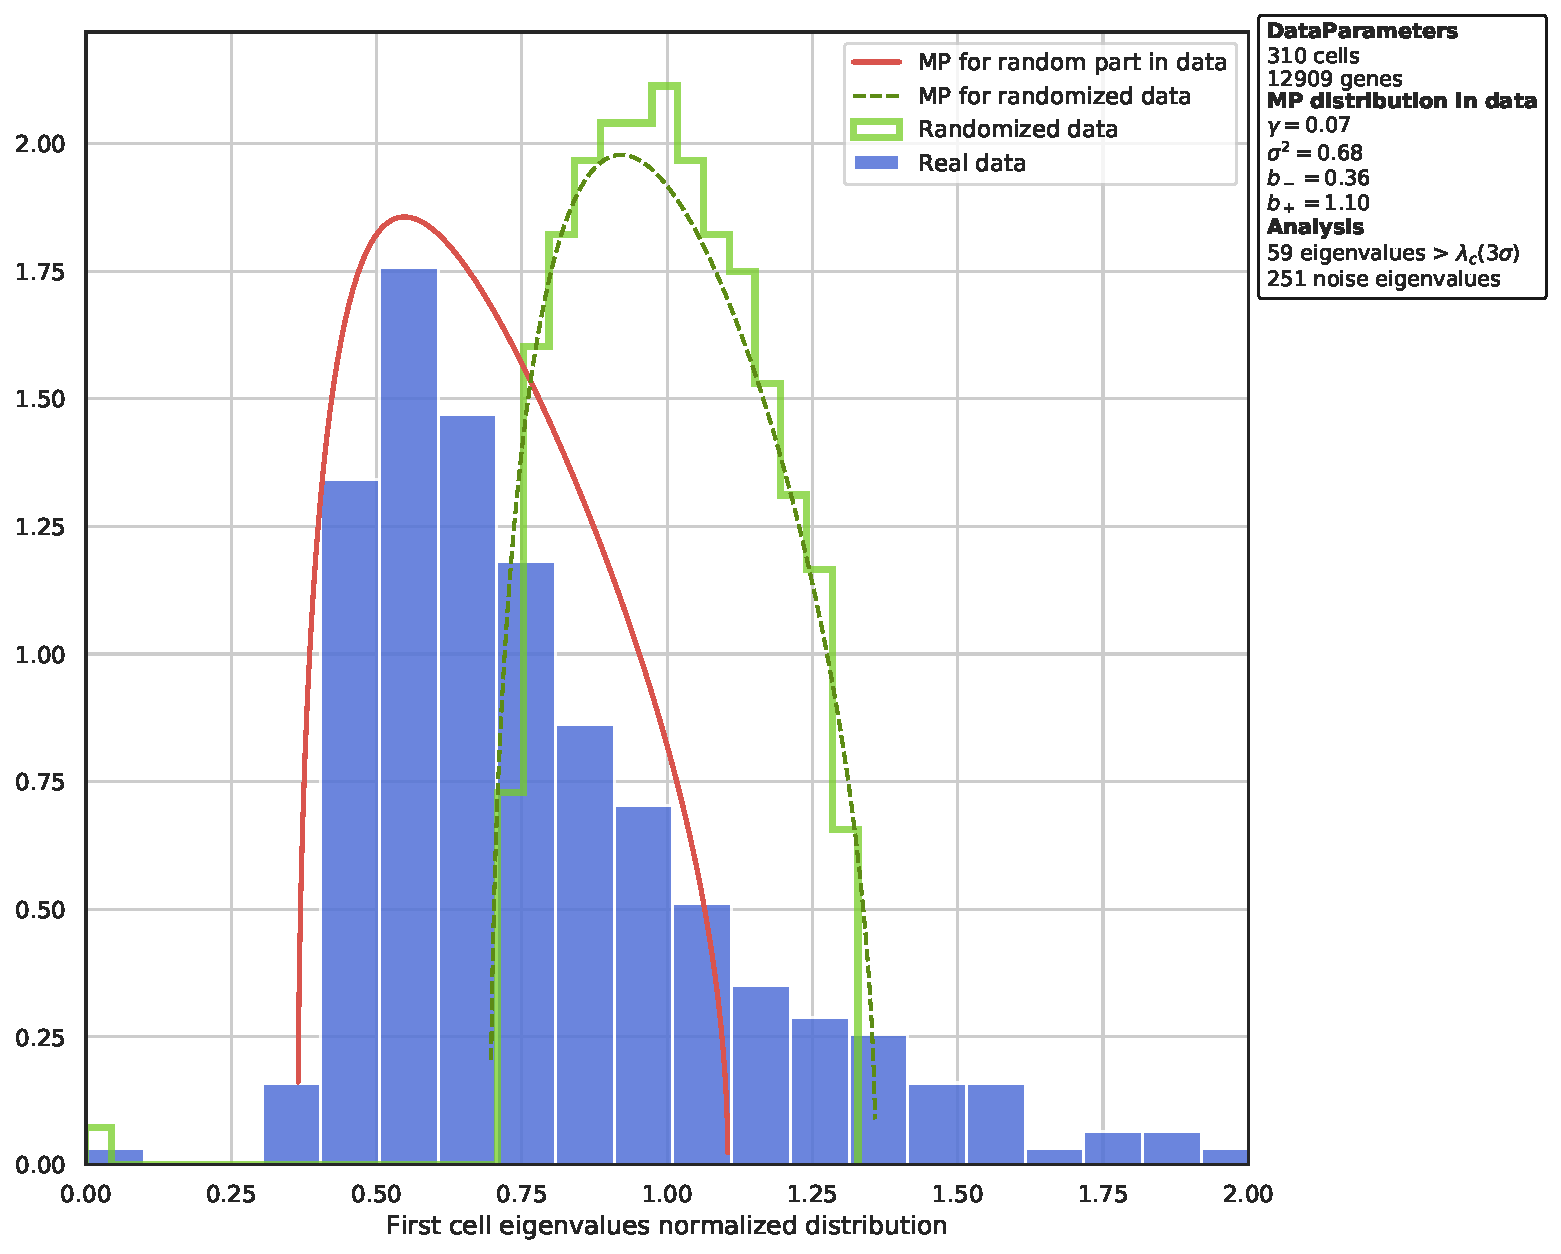
\includegraphics[scale=0.65]{mp_NC_HH1315}}
\caption{Distribution of eigenvalues of the cross-correlation matrix as calculated by the ``randomly'' software package \cite{Aparicio2018} for the single-cell RNAseq data from \cite{Morrison2017}. Bigger eigenvalues correspond to principal components that explain more variance of the data. Random matrix theory predicts that the eigenvalues of the cross-correlation matrix of a set of independent identically distributed random variables are distributed according to the Marchenko-Pastur law. Hence, a certain amount of correlation in a data-set is to be expected under the null model of independence, here shown in red, and only principal components with large enough eigenvalues are treated as signal (here, the top 59 eigenvalues). \label{figMP}}
\end{figure}

\begin{figure}
\centering
\subfloat[]{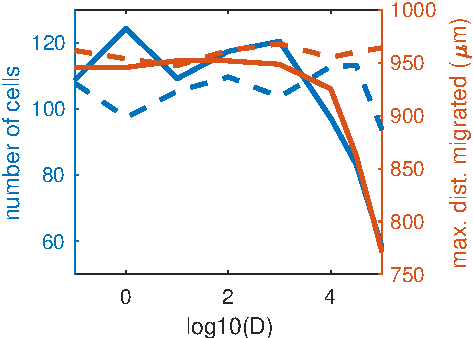
\includegraphics[]{FigS2_contStates_diffus_sensAcc_10}}\quad
\subfloat[]{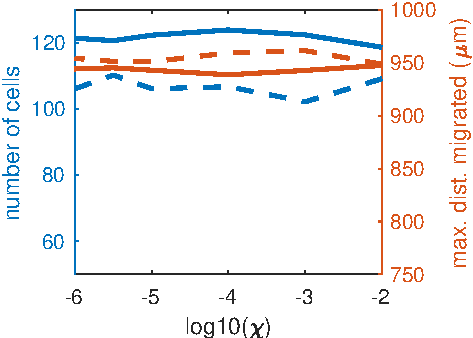
\includegraphics[]{FigS2_contStates_chi_sensAcc_10}}\\
\subfloat[]{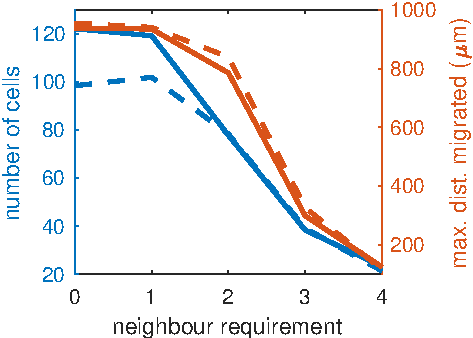
\includegraphics[]{FigS2_contStates_needNbrs_sensAcc_10}}
\caption{Further analysis of the continuous states model, showing total number of cells and maximum distance migrated after 18h of migration, varying (A) the chemoattractant diffusivity, D ($\mu m/h$), (B) the background chemoattractant production, $\chi$ (arbitrary units per hour), and (C)  introducing a neighbour requirement, such that cells only move in a directed manner if they have at least $n$ neighbours within filopodial reach. Data shown are averages over 40 repeated simulations for each parameter value.\label{figNaiveModelSweeps}}
\end{figure}

%%\paragraph{Fig. S3: additional simulation tests, eg transplant simulations}
\clearpage
\section*{References}
\bibliography{references}

\end{document}